\documentclass[conference]{IEEEtran}

\usepackage{cite}
\usepackage{graphicx}
\usepackage{booktabs}
\usepackage{array}
\usepackage{url}

\graphicspath{{../figures/}{reports/figures/}}

\begin{document}

\title{Comparing Deep Learning Models for Hotel Demand Forecasting and Dynamic Room Pricing}

\author{
\IEEEauthorblockN{Jack DeMarinis}
\IEEEauthorblockA{CSC 561 Final Project\\
United States\\
}
}

\maketitle

\begin{abstract}
This project develops an end-to-end hotel demand forecasting and pricing-support pipeline using real operational hotel data. Raw reservation, room-sales, and forecast reports are cleaned, deduplicated, audited, and converted into a daily modeling table covering 2023--2025. The main forecasting target is daily rooms sold. Classical baselines, tree-based tabular models, and neural sequence models are evaluated using chronological train, validation, and test splits. The primary reported model convention excludes operational rows flagged as known anomalies. XGBoost is the best model by test mean absolute error (MAE), achieving MAE 7.443, RMSE 9.927, and $R^2$ of 0.585 on the unflagged 2025 test period. Deep learning models are competitive but do not surpass the best tree models: the best GRU reaches MAE 7.813, and the best Transformer reaches MAE 7.835. A bounded pricing layer converts the selected XGBoost demand forecast into aggressive and conservative ADR recommendations. Under a static counterfactual that holds realized rooms sold fixed, the aggressive scenario increases simulated unflagged 2025 room revenue by \$88,101.38 and RevPAR by \$4.15, while the conservative scenario increases simulated revenue by \$44,092.35 and RevPAR by \$2.08. The results support a practical MVP conclusion: tree-based tabular forecasting remains the strongest approach for this small daily dataset, while GRU and Transformer models provide useful deep learning comparisons.
\end{abstract}

\begin{IEEEkeywords}
hotel demand forecasting, revenue management, XGBoost, random forest, GRU, LSTM, Transformer, dynamic pricing, interpretability
\end{IEEEkeywords}

\section{Introduction}
Hotels make pricing decisions under uncertainty: demand varies by day of week, season, events, booking behavior, room availability, and prior occupancy. Many small or independent hotel operations still rely on spreadsheets, manual review, or fixed pricing rules, even though commercial revenue management systems use data-driven demand signals to update prices more systematically. The goal of this project is to build an academic minimum viable product (MVP) that forecasts daily hotel demand and converts that forecast into bounded pricing recommendations.

The specific business setting is D.\ Hotel Suites \& Spa, an independent 60-room, six-floor hotel located in the Western Massachusetts area near Springfield, Massachusetts. The hotel serves a mix of regional leisure, business, and event-related travel demand. It was previously operated under the Country Inn \& Suites Holyoke flag and has since been rebranded as an independent property. Its inventory consists of regular rooms and suites totaling 60 rooms, and that 60-room capacity is used throughout the modeling and pricing pipeline.

The business motivation is direct: the property currently sets nightly rates manually using spreadsheets, historical reference rates, and operator judgment. There is no automated demand forecast and no automated pricing recommendation. This is a common constraint for independent hotels of this size, because commercial revenue management systems are often designed for larger chains and can be expensive to integrate for a single property. I built this MVP as a lower-cost, human-approved decision-support system that uses the same operational reports the hotel already produces.

I have access to the property's operational reports through a family connection with a partner at the hotel, which allowed me to use a real single-property dataset rather than a public benchmark. From a machine learning perspective, the task is a structured time-series regression problem. From a business perspective, it is a pricing-support problem where prediction errors and recommendation constraints both matter. The project therefore evaluates predictive performance using MAE, RMSE, MAPE, and $R^2$, and evaluates pricing support using static revenue, ADR, occupancy, and RevPAR metrics.

The proposal emphasized comparison between classical machine learning and deep learning architectures. This report implements that comparison using simple time-series baselines, Ridge regression, Random Forests \cite{breiman2001random}, XGBoost \cite{chen2016xgboost}, MLP models, LSTM models \cite{hochreiter1997lstm}, GRU models \cite{cho2014gru}, and small Transformer encoders \cite{vaswani2017attention}. The final system uses a two-stage pipeline: first forecast demand, then apply bounded pricing rules.

\section{Data Sources}
The data were taken from actual operational workbooks exported from the hotel's reservations and reporting system. The raw sources include reservation-style guest reports, Block RoomSales reports, and ReservationForecast reports. These are internal hotel reports rather than simulated or public benchmark data.

The final modeling table contains 1,096 daily rows and 209 columns covering January 1, 2023 through December 31, 2025. The table is date-grain: each row represents one business date. It joins cleaned room-sales history, reservation forecast fields, and guest-arrival enrichment. The primary forecasting target is daily rooms sold.

Cleaning included parsing multi-line guest report blocks, standardizing dates and numeric fields, normalizing key text values, preserving source lineage, and removing duplicates with an auditable deduplication process. The data quality audit flagged two over-capacity rows and twelve zero-room-sold rows. These rows are retained for traceability, but the primary reported model convention excludes all flagged dates because they are known operational anomalies.

Fig.~\ref{fig:pipeline} summarizes the final pipeline.

\begin{figure*}[t]
    \centering
    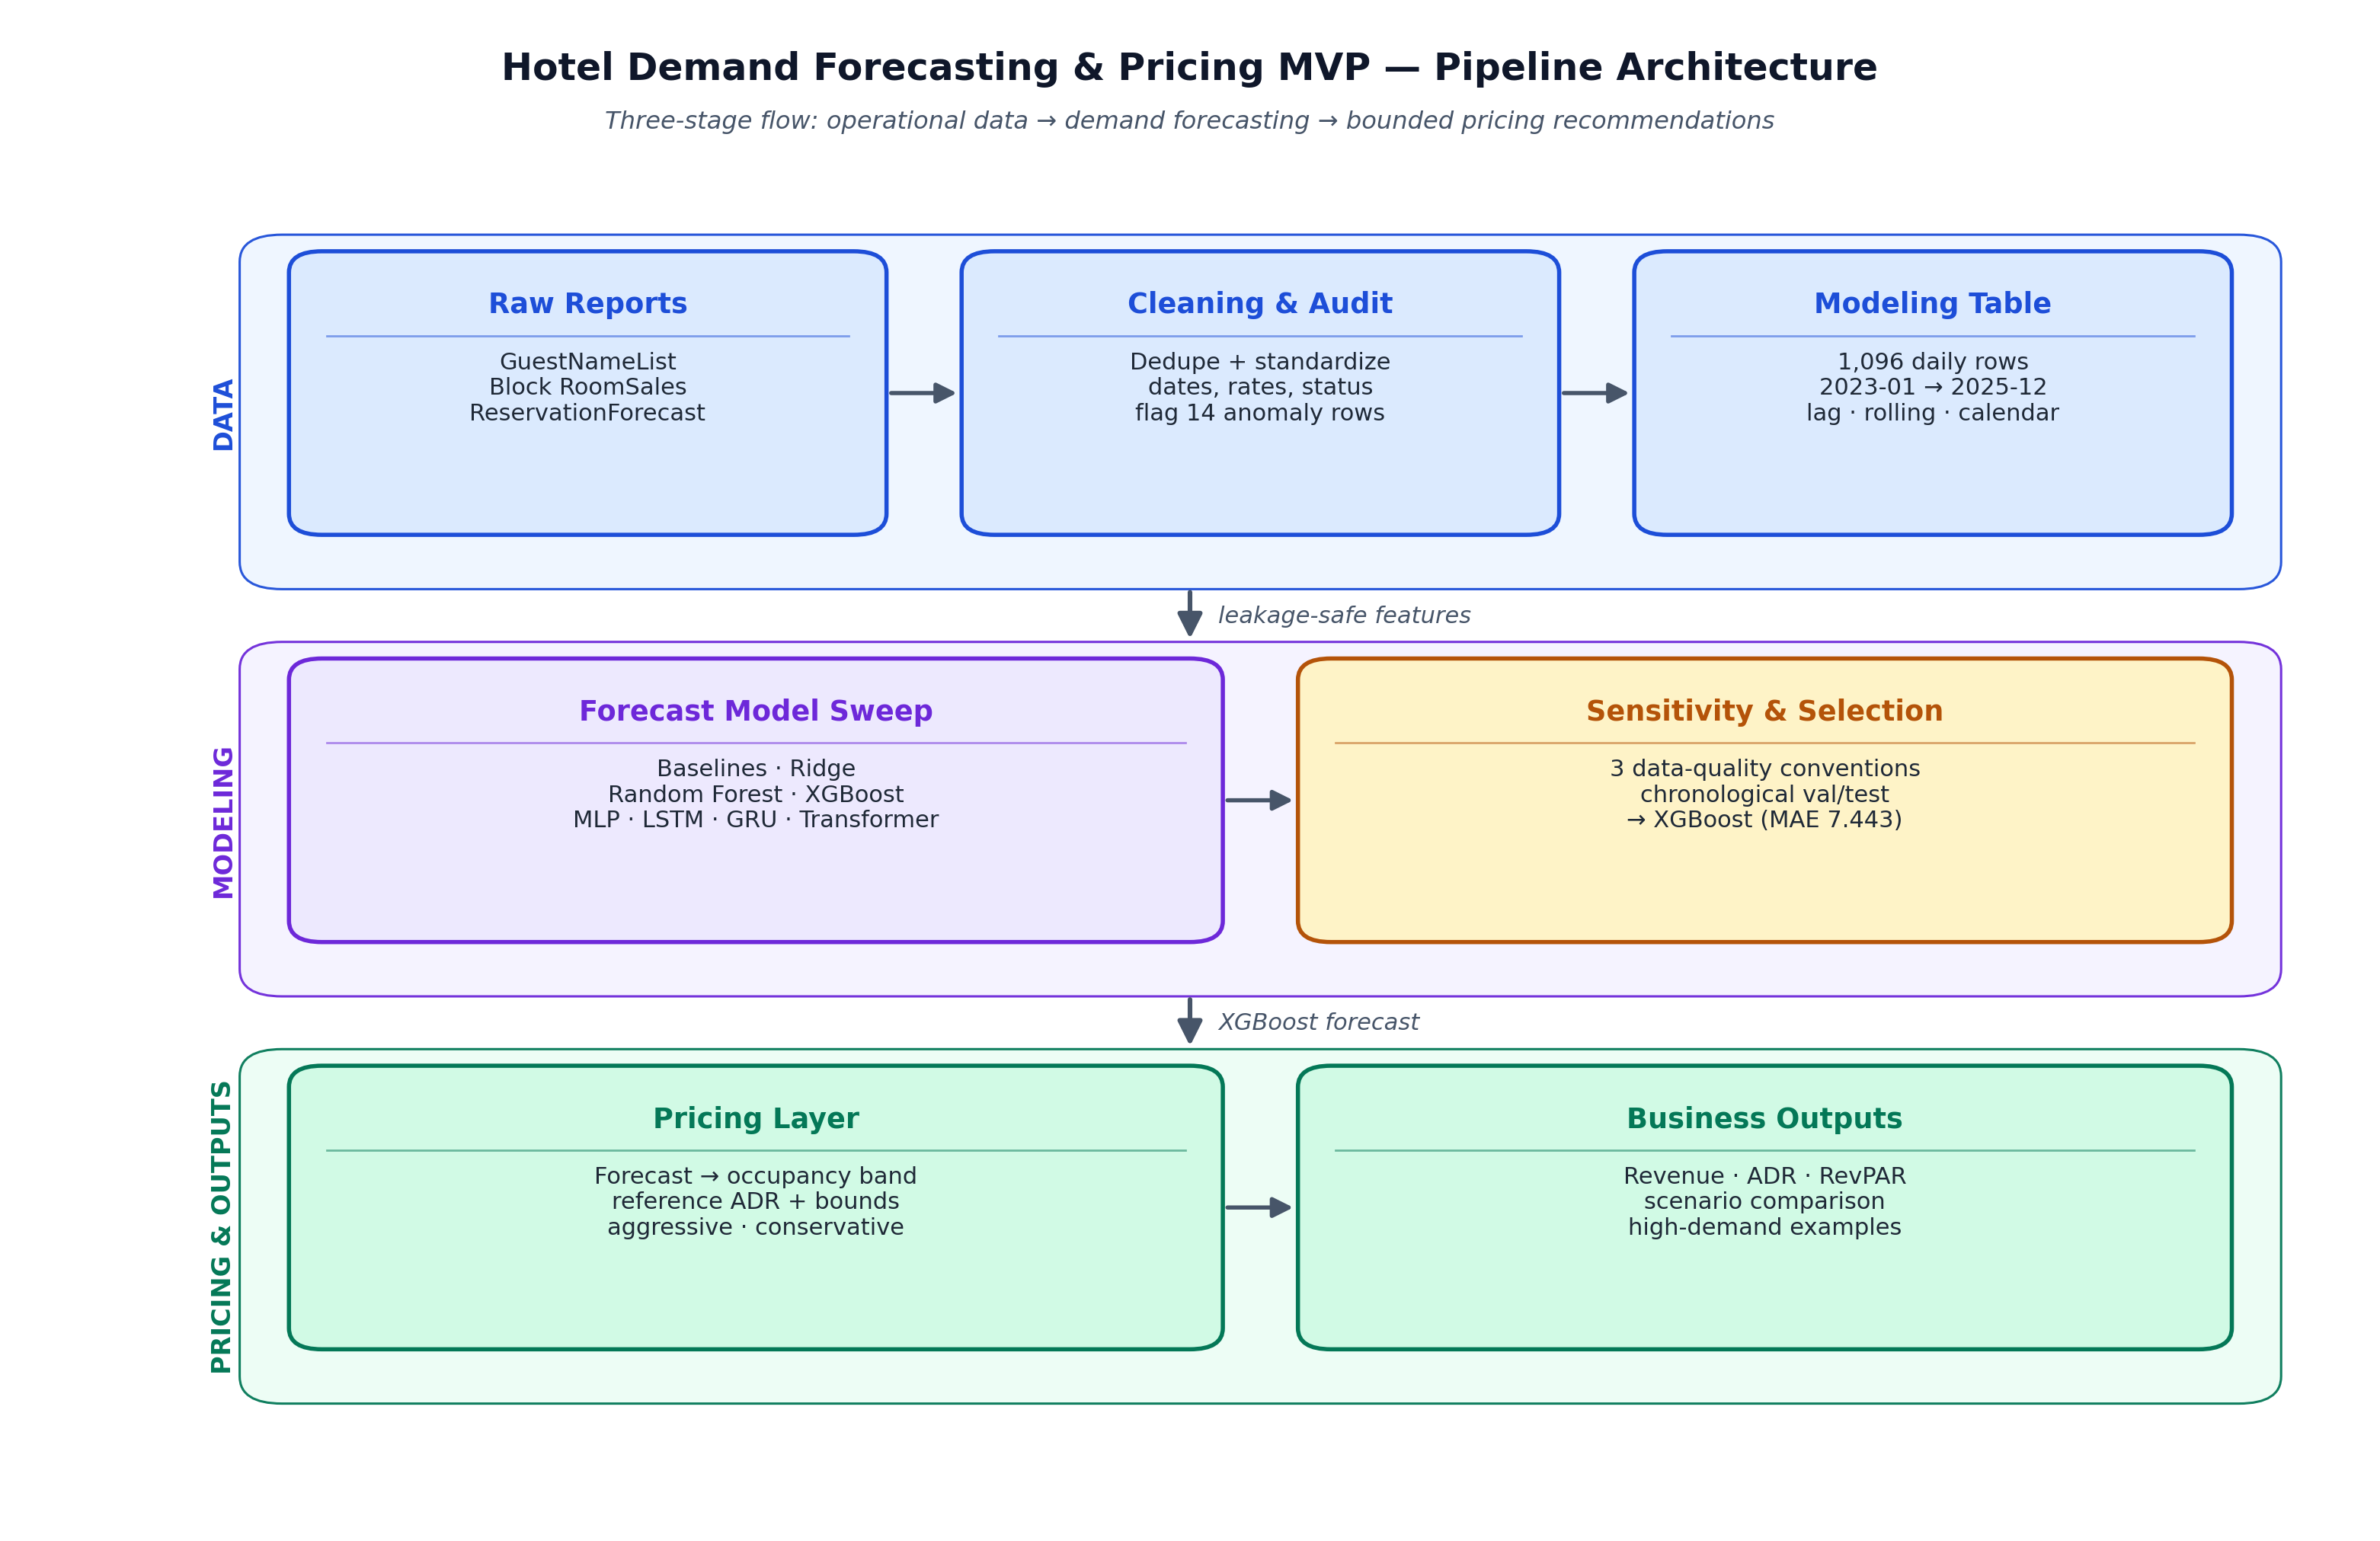
\includegraphics[width=0.96\textwidth]{final_pipeline_architecture.png}
    \caption{End-to-end hotel demand forecasting and pricing MVP pipeline.}
    \label{fig:pipeline}
\end{figure*}

\section{Feature Engineering}
Features were designed to be forecast-oriented and leakage-safe. Same-day operational fields, same-day guest enrichment fields, and raw future ReservationForecast fields were excluded from learned model inputs. The model inputs combine:
\begin{itemize}
    \item calendar features such as day of week, month, quarter, weekend flags, and cyclical encodings;
    \item lagged historical values for rooms sold, ADR, revenue, and occupancy;
    \item rolling means, medians, and standard deviations over 7, 14, 28, and 56 day windows;
    \item derived comparisons such as week-over-week changes.
\end{itemize}

All rolling features are shifted so that the current day's target is not included in the feature values. This matters because the intended use case is forecasting before final realized demand is known.

\section{Models and Evaluation}
\subsection{Splitting Strategy}
The dataset is split chronologically. Training uses January 1, 2023 through June 30, 2024; validation uses July 1, 2024 through December 31, 2024; and testing uses calendar year 2025. This matches the operational goal of generalizing to a later time period.

Three data-quality conventions are reported. The full-data reference uses all rows. The over-capacity sensitivity removes only rows where rooms sold exceeded inferred capacity. The primary anomaly-excluded convention drops every row tagged by the data-quality audit, and is the convention used for the headline results throughout the paper.

\subsection{Classical and Tree-Based Models}
Baselines include previous-day demand, previous-week demand, rolling averages, and Ridge regression. Tree-based tabular models include Random Forest and XGBoost. The implementation uses scikit-learn \cite{pedregosa2011scikit} and XGBoost.

Table~\ref{tab:baseline} shows the full-data 2025 test results. XGBoost is best by MAE, while Random Forest has slightly stronger RMSE and $R^2$. MAPE values should be read with care: the property has only 60 rooms and the test period contains several low-demand and near-zero-demand dates, so MAPE is sensitive to small denominators and tends to look pessimistic relative to absolute-error metrics. MAE and RMSE are therefore treated as the primary comparison metrics in this report, with MAPE reported for completeness.

\begin{table}[t]
\centering
\caption{Full-Data 2025 Test Metrics}
\label{tab:baseline}
\begin{tabular}{lrrrrr}
\toprule
Model & Rows & MAE & RMSE & MAPE (\%) & $R^2$\\
\midrule
XGBoost & 365 & 8.039 & 11.210 & 45.42 & 0.539\\
Random Forest & 365 & 8.062 & 10.870 & 42.36 & 0.567\\
Previous Week & 365 & 9.551 & 13.438 & 35.02 & 0.338\\
Previous Day & 365 & 11.307 & 15.987 & 42.01 & 0.063\\
Rolling 7d & 365 & 12.528 & 15.107 & 44.45 & 0.164\\
Ridge & 365 & 12.744 & 14.938 & 52.08 & 0.182\\
Rolling 28d & 365 & 13.511 & 16.073 & 52.46 & 0.053\\
\bottomrule
\end{tabular}
\end{table}

Table~\ref{tab:sensitivity} shows the sensitivity analysis. The primary report result is XGBoost under the anomaly-excluded convention: MAE 7.443, RMSE 9.927, and $R^2$ 0.585.

\begin{table}[t]
\centering
\caption{Best Learned Model by Data-Quality Convention}
\label{tab:sensitivity}
\resizebox{\columnwidth}{!}{%
\begin{tabular}{llrrrrr}
\toprule
Scenario & Model & Rows & MAE & RMSE & MAPE (\%) & $R^2$\\
\midrule
All flags excl. & XGBoost & 354 & 7.443 & 9.927 & 45.62 & 0.585\\
Over-cap excl. & RF & 365 & 8.019 & 10.757 & 41.61 & 0.576\\
Full data & XGBoost & 365 & 8.039 & 11.210 & 45.42 & 0.539\\
\bottomrule
\end{tabular}}
\end{table}

Fig.~\ref{fig:predicted_vs_actual} compares predicted and actual daily rooms sold across the 2025 test period for XGBoost, Random Forest, and the two strongest heuristic baselines. The learned tabular models track the weekly seasonal cycle and high-occupancy weekends closely; the heuristic baselines either lag the signal (previous-day) or smooth out short-term swings (previous-week).

\begin{figure}[t]
    \centering
    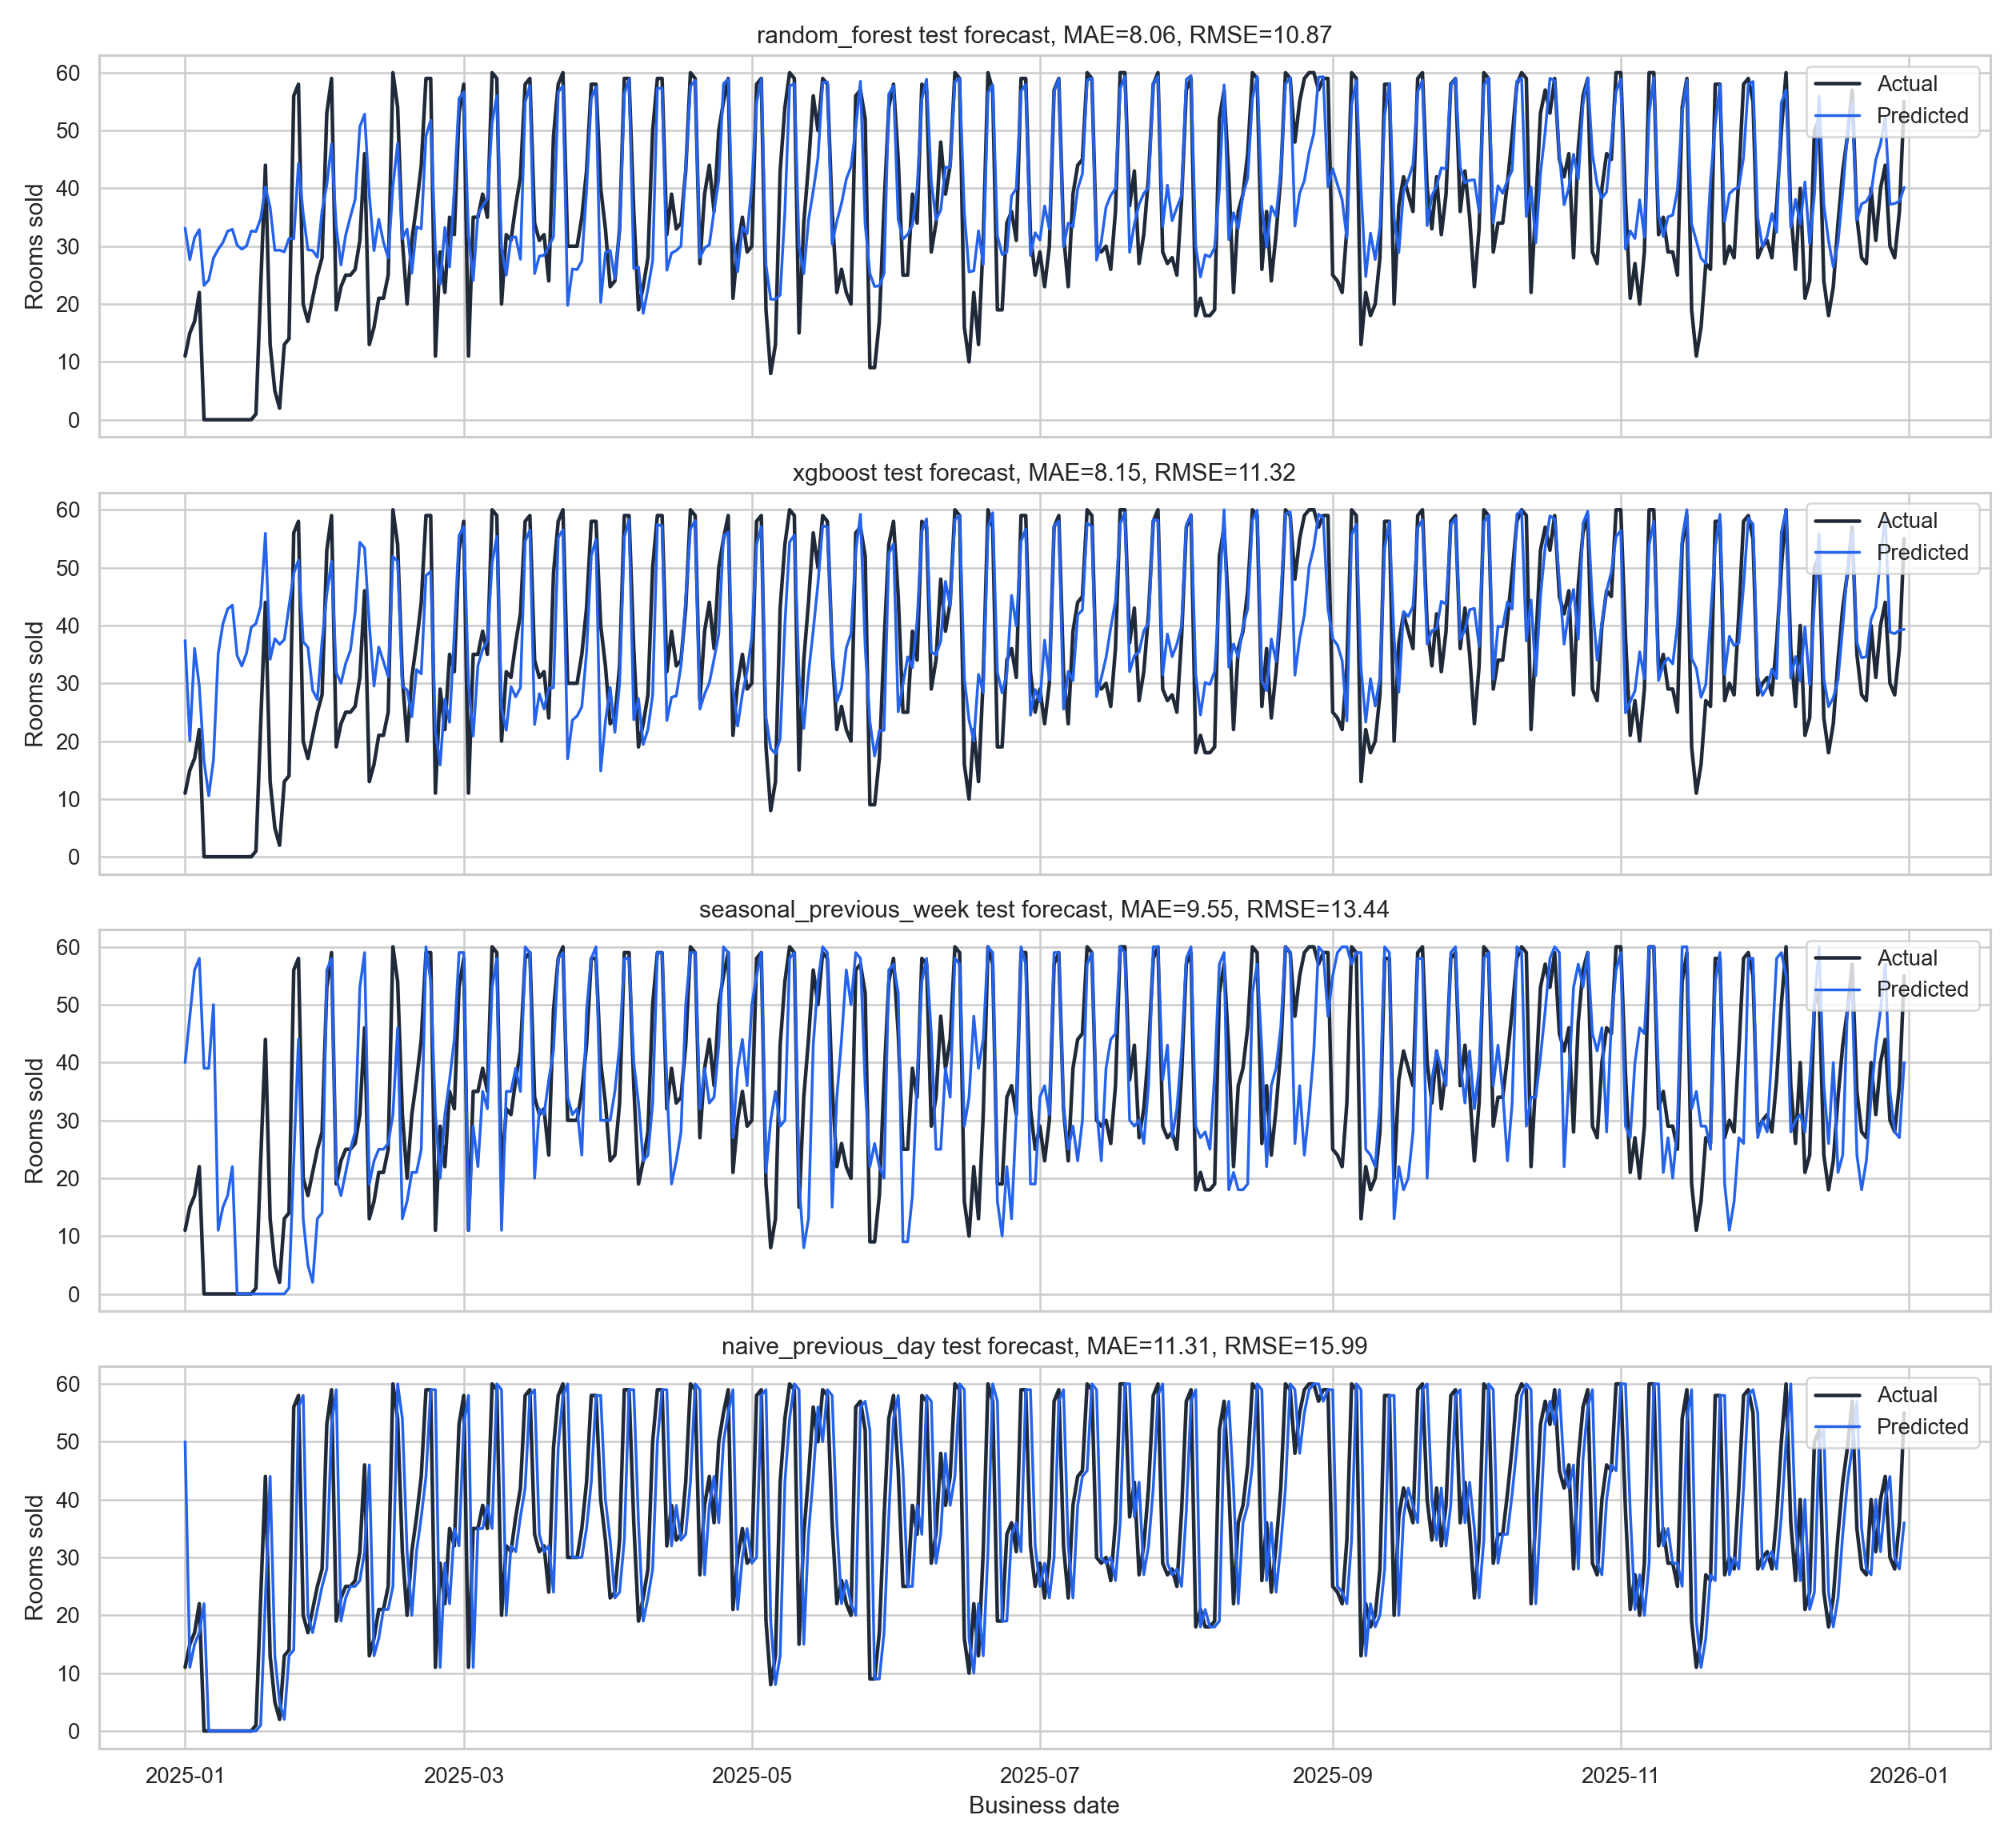
\includegraphics[width=\columnwidth]{baseline_predicted_vs_actual_test.png}
    \caption{Predicted versus actual daily rooms sold over the full 2025 test period for the strongest tabular models and two reference baselines.}
    \label{fig:predicted_vs_actual}
\end{figure}

\subsection{Deep Learning Models}
The deep learning comparison includes tabular MLP models and sequence models. LSTM, GRU, and Transformer candidates use sequential windows ending on each prediction date. PyTorch \cite{paszke2019pytorch} is used for LSTM, GRU, and Transformer training, with AdamW optimization \cite{loshchilov2019adamw}, Smooth L1 loss, gradient clipping, and early stopping on validation loss.

\subsubsection{Hyperparameter Sweep}
Fourteen configurations were trained across the four families: three MLP variants, three LSTM variants, six GRU variants, and two Transformer variants. The search axes are summarized in Table~\ref{tab:hyperparams}. Lookback length was the primary search axis for the sequence models. All sequence configurations use one recurrent (or Transformer) layer; Transformer variants use four attention heads. Dropout is zero for LSTM and GRU and 0.10--0.15 for Transformer. Patience for early stopping ranges from 90 to 120 epochs depending on the configuration. Targets and feature inputs are standardized before training. The sweep is intentionally scoped: the goal is an honest comparison rather than an exhaustive neural architecture search.

\begin{table}[t]
\centering
\caption{Deep Learning Hyperparameter Sweep}
\label{tab:hyperparams}
\resizebox{\columnwidth}{!}{%
\begin{tabular}{llllr}
\toprule
Family & Lookback (days) & Hidden size & Learning rate & Configs\\
\midrule
MLP         & --                       & (32), (64,32)        & 0.0007--0.001  & 3\\
LSTM        & 14, 28, 56               & 32, 48, 64           & 0.0005--0.001  & 3\\
GRU         & 14, 28, 42, 56, 84       & 32, 48, 64           & 0.0005--0.001  & 6\\
Transformer & 28, 56                   & 48, 64 (4 heads)     & 0.0004--0.0005 & 2\\
\bottomrule
\end{tabular}}
\end{table}

\subsubsection{Headline Results}
Table~\ref{tab:deep} compares the strongest model from each architecture family under the primary anomaly-excluded test convention, including all four deep learning architectures from the proposal. The best GRU reaches MAE 7.813, and the best Transformer reaches MAE 7.835. The best LSTM reaches MAE 8.662, and the best MLP only reaches MAE 12.663 with a negative $R^2$, indicating that purely tabular MLPs do not generalize on this small dataset.

\begin{table}[t]
\centering
\caption{Best Model per Family on Unflagged 2025 Test Rows}
\label{tab:deep}
\resizebox{\columnwidth}{!}{%
\begin{tabular}{lrrrrr}
\toprule
Model & Rows & MAE & RMSE & MAPE (\%) & $R^2$\\
\midrule
XGBoost & 354 & 7.443 & 9.927 & 45.62 & 0.585\\
Random Forest & 354 & 7.466 & 9.834 & 42.67 & 0.593\\
GRU 56d wide & 354 & 7.813 & 10.588 & 48.82 & 0.528\\
Transformer 28d & 354 & 7.835 & 10.305 & 43.23 & 0.553\\
LSTM 56d & 354 & 8.662 & 11.210 & 51.68 & 0.471\\
MLP medium & 354 & 12.663 & 16.631 & 64.36 & $-$0.165\\
\bottomrule
\end{tabular}}
\end{table}

\subsubsection{Statistical Significance}
The point-estimate MAE differences between XGBoost and the strongest sequence models are small relative to the size of the test set, so the headline ranking deserves a statistical check. Table~\ref{tab:bootstrap} reports paired bootstrap 95\% confidence intervals on the test MAE difference (other model minus XGBoost) using 10,000 resamples of the 354-row unflagged 2025 test set, drawn with replacement at the date level. The Random Forest, best GRU, and best Transformer intervals all span zero, so under this paired date-level bootstrap the XGBoost advantage over those models is not statistically distinguishable on this test set. Only the best LSTM and the best MLP intervals exclude zero, meaning XGBoost is significantly better than those families at 95\% confidence under the same procedure but only nominally better than Random Forest, GRU, and Transformer. This is the more accurate way to read Table~\ref{tab:deep}: under this paired date-level bootstrap the strong tree and best sequence models form a statistical tie, while LSTM and MLP variants tested here trail meaningfully.

\begin{table}[t]
\centering
\caption{Paired Bootstrap 95\% CIs vs.\ XGBoost (10,000 Resamples, 354 Rows)}
\label{tab:bootstrap}
\begin{tabular}{lrr}
\toprule
Comparison & $\Delta$MAE & 95\% CI\\
\midrule
Random Forest    & $+0.023$ & $[-0.315,\ +0.349]$\\
Best GRU         & $+0.369$ & $[-0.203,\ +0.925]$\\
Best Transformer & $+0.392$ & $[-0.215,\ +0.978]$\\
Best LSTM        & $+1.219$ & $[+0.656,\ +1.789]$\\
Best MLP         & $+5.220$ & $[+4.090,\ +6.324]$\\
\bottomrule
\end{tabular}
\end{table}

Fig.~\ref{fig:deep} visualizes the model comparison. The honest interpretation is that sequence neural networks are statistically competitive with tree-based tabular models on this dataset, but the available sample size does not give a sequence architecture a significant advantage over XGBoost. The deep learning hypothesis from the proposal is therefore supported in part: GRU and Transformer match the strongest tabular baselines, but they do not surpass them.

\begin{figure}[t]
    \centering
    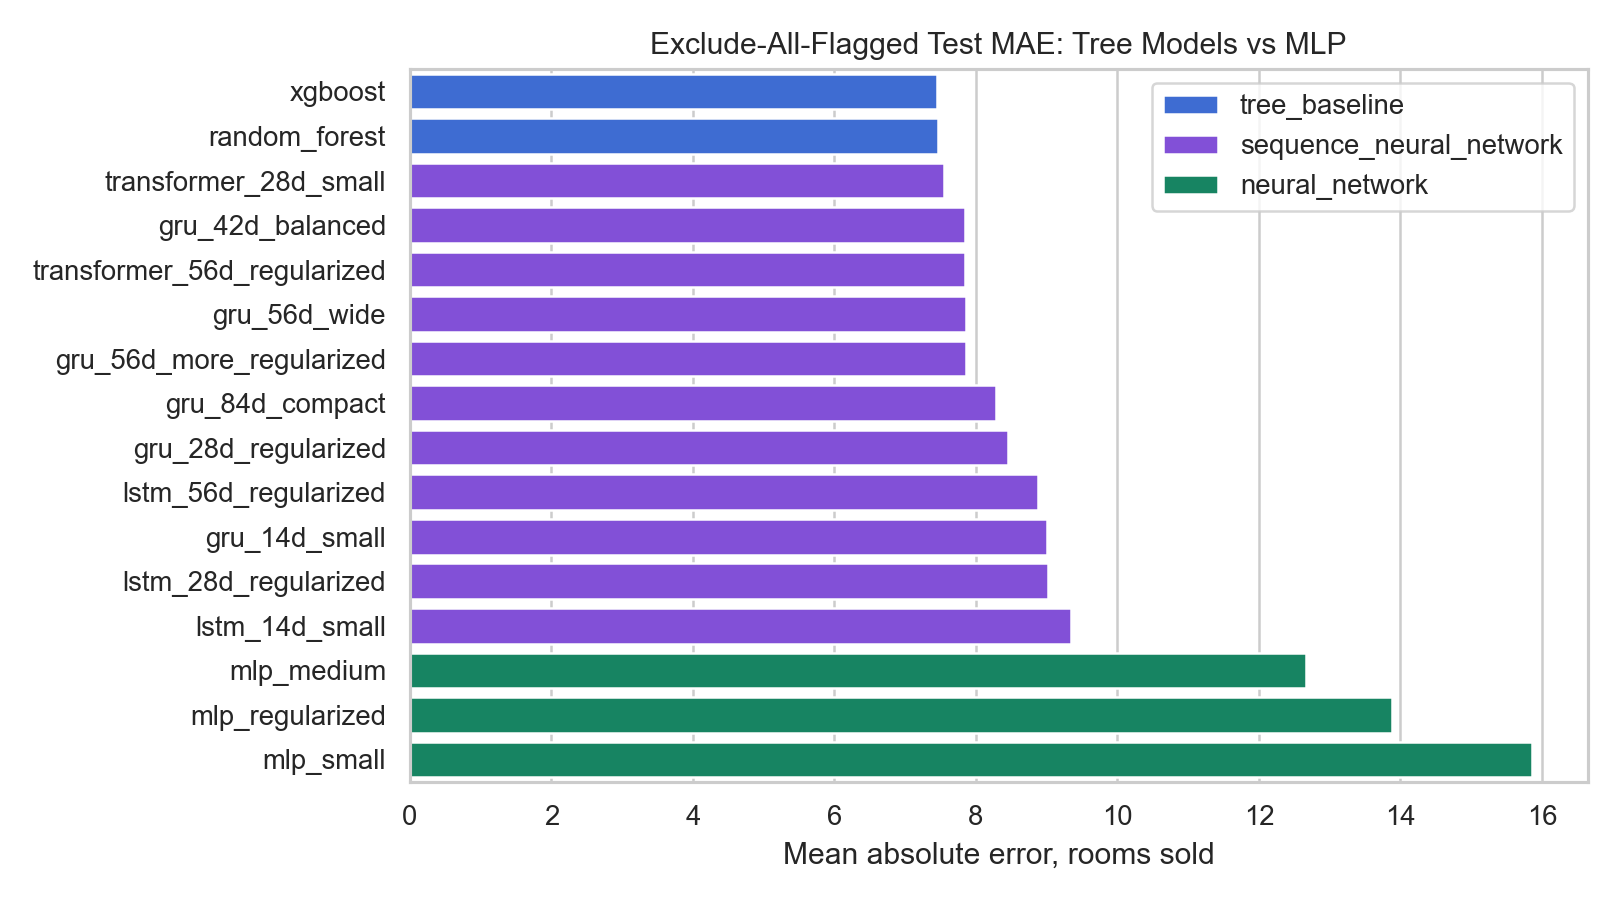
\includegraphics[width=\columnwidth]{deep_learning_model_comparison.png}
    \caption{Exclude-all-flagged test MAE comparison across tree and neural models.}
    \label{fig:deep}
\end{figure}

\section{Feature Importance}
The XGBoost feature-importance analysis shows that recent weekly history is the strongest signal. The top features are the seven-day and fourteen-day lags of rooms sold, the seven-day lag of net room revenue, the day-of-week encoding, and the one-day lag of net room revenue. This is consistent with the domain expectation that hotel demand has strong weekly seasonality and short-term persistence.

\begin{figure}[t]
    \centering
    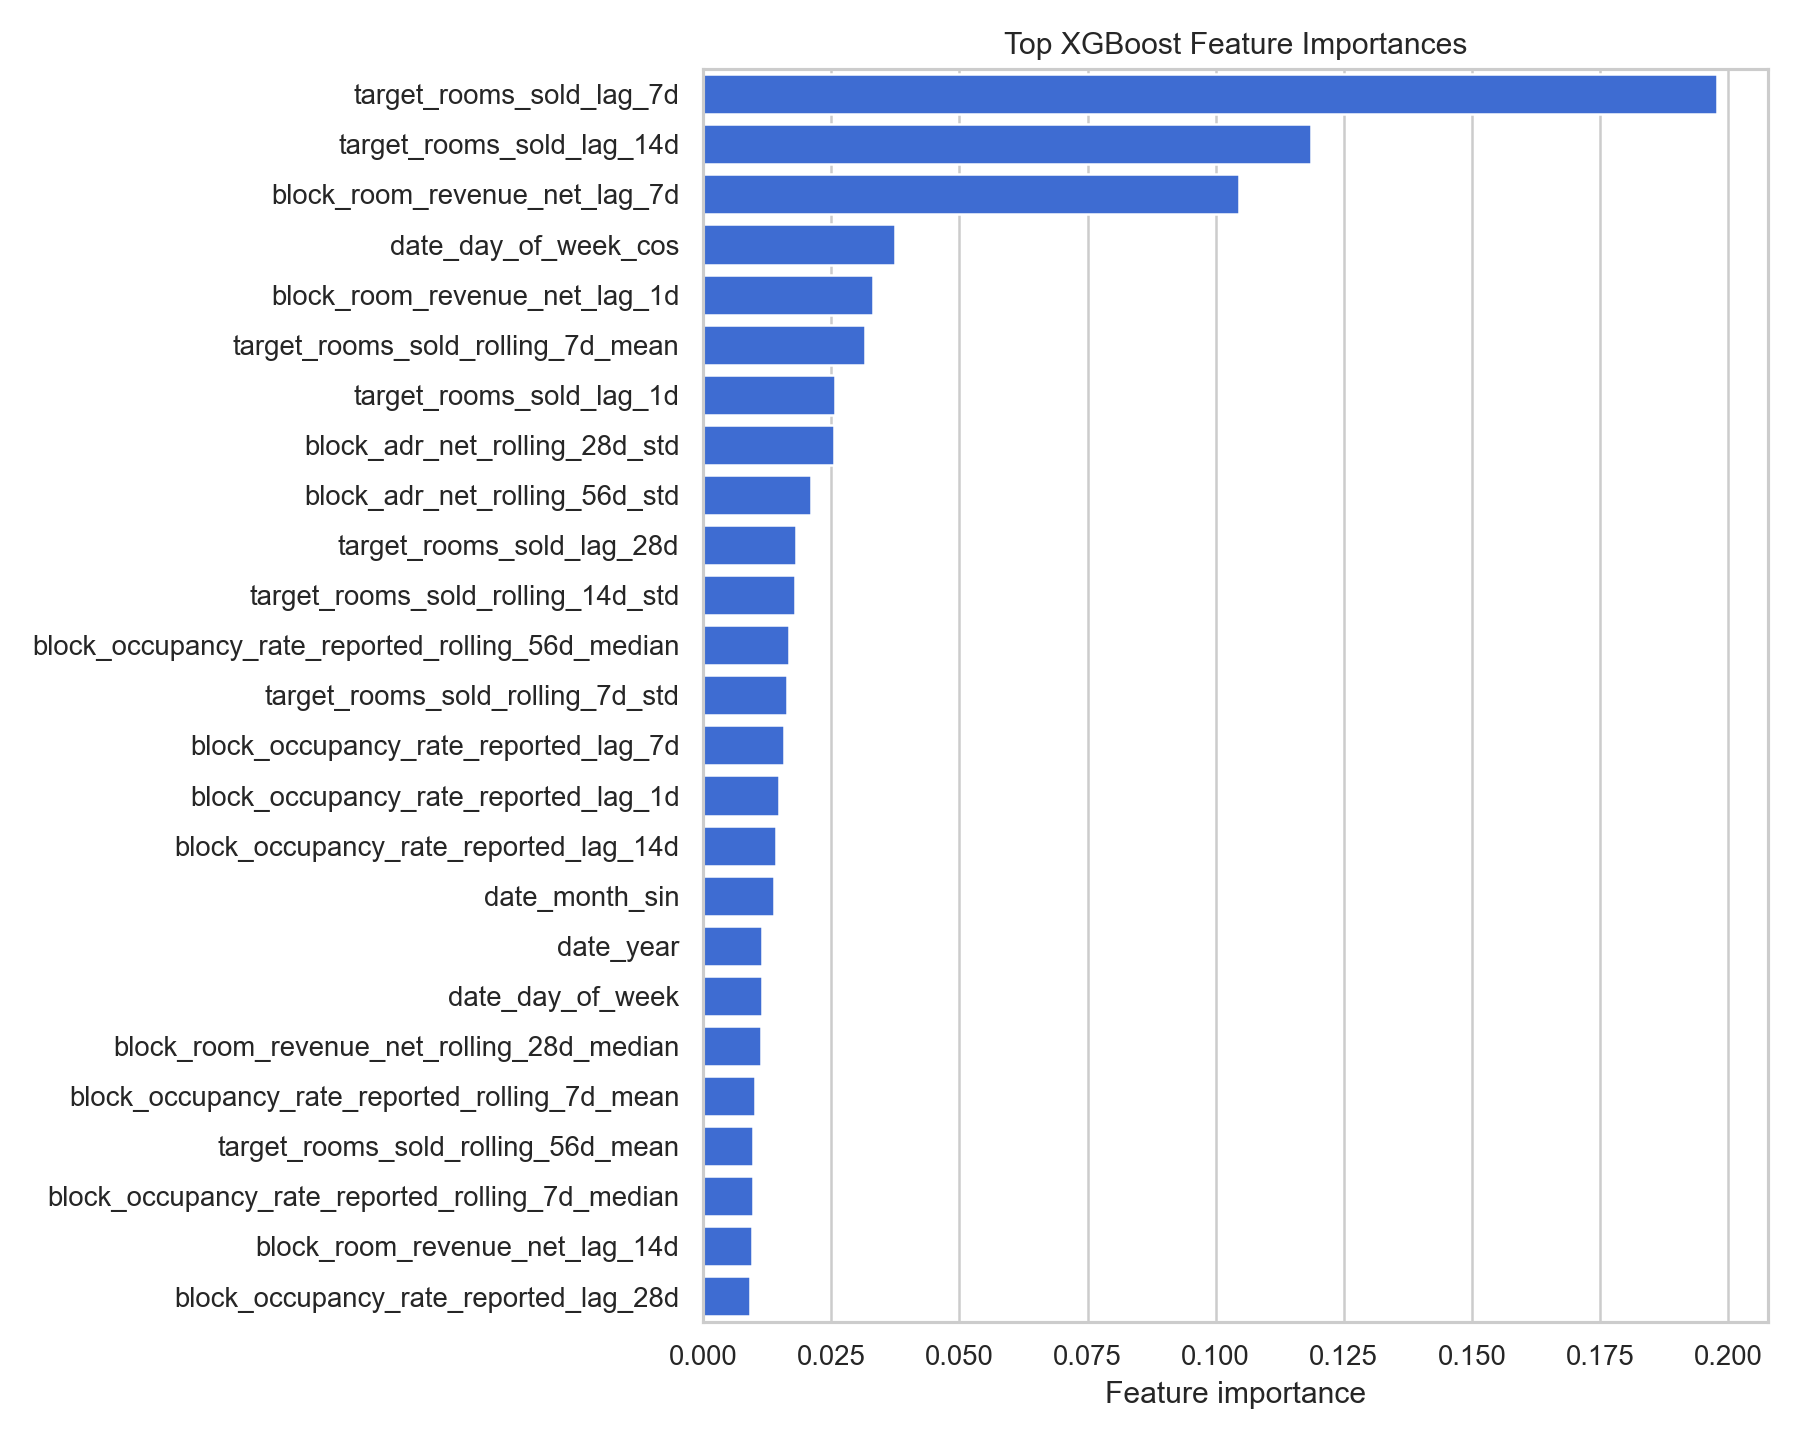
\includegraphics[width=\columnwidth]{xgboost_feature_importance.png}
    \caption{Top XGBoost feature importances under the primary training setup.}
    \label{fig:importance}
\end{figure}

\section{Interpretability and Model Choice}
Under the paired date-level bootstrap reported in Table~\ref{tab:bootstrap}, XGBoost, Random Forest, the best GRU, and the best Transformer are statistically indistinguishable on test MAE. When predictive accuracy is indistinguishable, principled model selection requires a second axis. For a pricing-support MVP that surfaces ADR recommendations to a human revenue manager, that second axis is interpretability: a recommendation is operationally useful only if the manager can audit why the model is asking to raise or lower the rate, and an unexplained ADR change is hard to distinguish from a guess. This framing follows the position taken in high-stakes interpretable-ML work \cite{rudin2019stopblackbox}, which argues that models affecting real-world decisions should be inherently or post-hoc explainable rather than treated as opaque oracles.

The model families differ substantially on this axis. The heuristic baselines are trivially interpretable but are too inaccurate for production use. Ridge regression provides global linear coefficients but underperforms by a wide margin and cannot capture the nonlinear interactions present in hotel demand. Random Forest and XGBoost are tree ensembles whose individual trees are inspectable and which support mature post-hoc explanation tools: feature importance, partial dependence, and local Shapley-value attributions \cite{lundberg2017shap} that map any single prediction back to the features that drove it. The MLP, LSTM, and GRU sequence models are less directly interpretable: post-hoc methods such as permutation importance, LIME \cite{ribeiro2016lime}, integrated gradients, and SHAP applied to the neural model are possible but require additional engineering, and their explanations are noisier on a 1,096-row dataset. Transformer attention weights provide a partial view of which past timesteps the model attends to, but attention is not a direct substitute for feature attribution.

Combining the bootstrap and interpretability views resolves the model choice more cleanly than the raw MAE table alone suggests. XGBoost is statistically tied with the strongest sequence models on accuracy but is materially more transparent. The feature-importance result in Fig.~\ref{fig:importance} already shows that the model's strongest signals are seven-day and fourteen-day lagged rooms sold, lagged room revenue, and day-of-week encoding --- features a hotel manager would recognize as the same signals they themselves use, which is a useful sanity check on the model's logic. A SHAP-based per-prediction explanation could be added without retraining, because tree-specific SHAP implementations exist for XGBoost. The same level of explanation would require additional engineering for the GRU or Transformer with no accuracy gain in return. Under the criterion that the model must support human-approved pricing decisions, the tie among XGBoost, GRU, and Transformer on accuracy resolves in favor of XGBoost on interpretability. The recommended choice is therefore not "XGBoost wins by MAE" but "XGBoost is the right operational choice because it is statistically as accurate as the best sequence models while being more auditable for a revenue manager."

\section{Pricing Recommendation Layer}
The pricing layer uses the selected XGBoost forecast. Forecast occupancy is computed as forecast rooms sold divided by total property rooms. A reference ADR is chosen from historical same-day ADR with rolling and lagged ADR fallbacks. The pricing rule then applies bounded demand-based adjustments.

Two scenarios are evaluated. The aggressive scenario uses 4\%, 8\%, and 12\% adjustment bands. The conservative scenario uses 2\%, 4\%, and 6\% bands. ADR is also bounded by minimum and maximum ADR constraints and by a maximum daily change from the reference ADR.

The pricing simulation is intentionally static. It applies recommended ADR to actual realized rooms sold and does not estimate price elasticity, competitor reaction, or occupancy changes caused by price changes. This makes the result a useful academic counterfactual, not proof of actual achievable revenue.

Table~\ref{tab:pricing} shows static unflagged 2025 pricing results. The aggressive scenario produces a simulated revenue lift of \$88,101.38, while the conservative scenario produces \$44,092.35.

\begin{table}[t]
\centering
\caption{Static Pricing Scenario Results on Unflagged 2025 Test Days}
\label{tab:pricing}
\begin{tabular}{lrrrr}
\toprule
Scenario & Hist. Rev. & Sim. Rev. & Delta & Delta \%\\
\midrule
Aggressive & \$2.018M & \$2.106M & \$88.1K & 4.37\%\\
Conservative & \$2.018M & \$2.062M & \$44.1K & 2.18\%\\
\bottomrule
\end{tabular}
\end{table}

Table~\ref{tab:business} adds occupancy and RevPAR context. Static occupancy delta is zero by design because rooms sold are held fixed. RevPAR improves by \$4.15 in the aggressive scenario and \$2.08 in the conservative scenario.

\begin{table}[t]
\centering
\caption{Business Metrics on Unflagged 2025 Test Days}
\label{tab:business}
\resizebox{\columnwidth}{!}{%
\begin{tabular}{lrrrr}
\toprule
Scenario & Act. Occ. & Fcst. Occ. & Hist. RevPAR & Sim. RevPAR\\
\midrule
Aggressive & 63.63\% & 66.13\% & \$95.01 & \$99.16\\
Conservative & 63.63\% & 66.13\% & \$95.01 & \$97.09\\
\bottomrule
\end{tabular}
}
\end{table}

Fig.~\ref{fig:adr} compares historical and recommended ADR over time. Fig.~\ref{fig:scenario} compares the aggressive and conservative revenue deltas.

\begin{figure}[t]
    \centering
    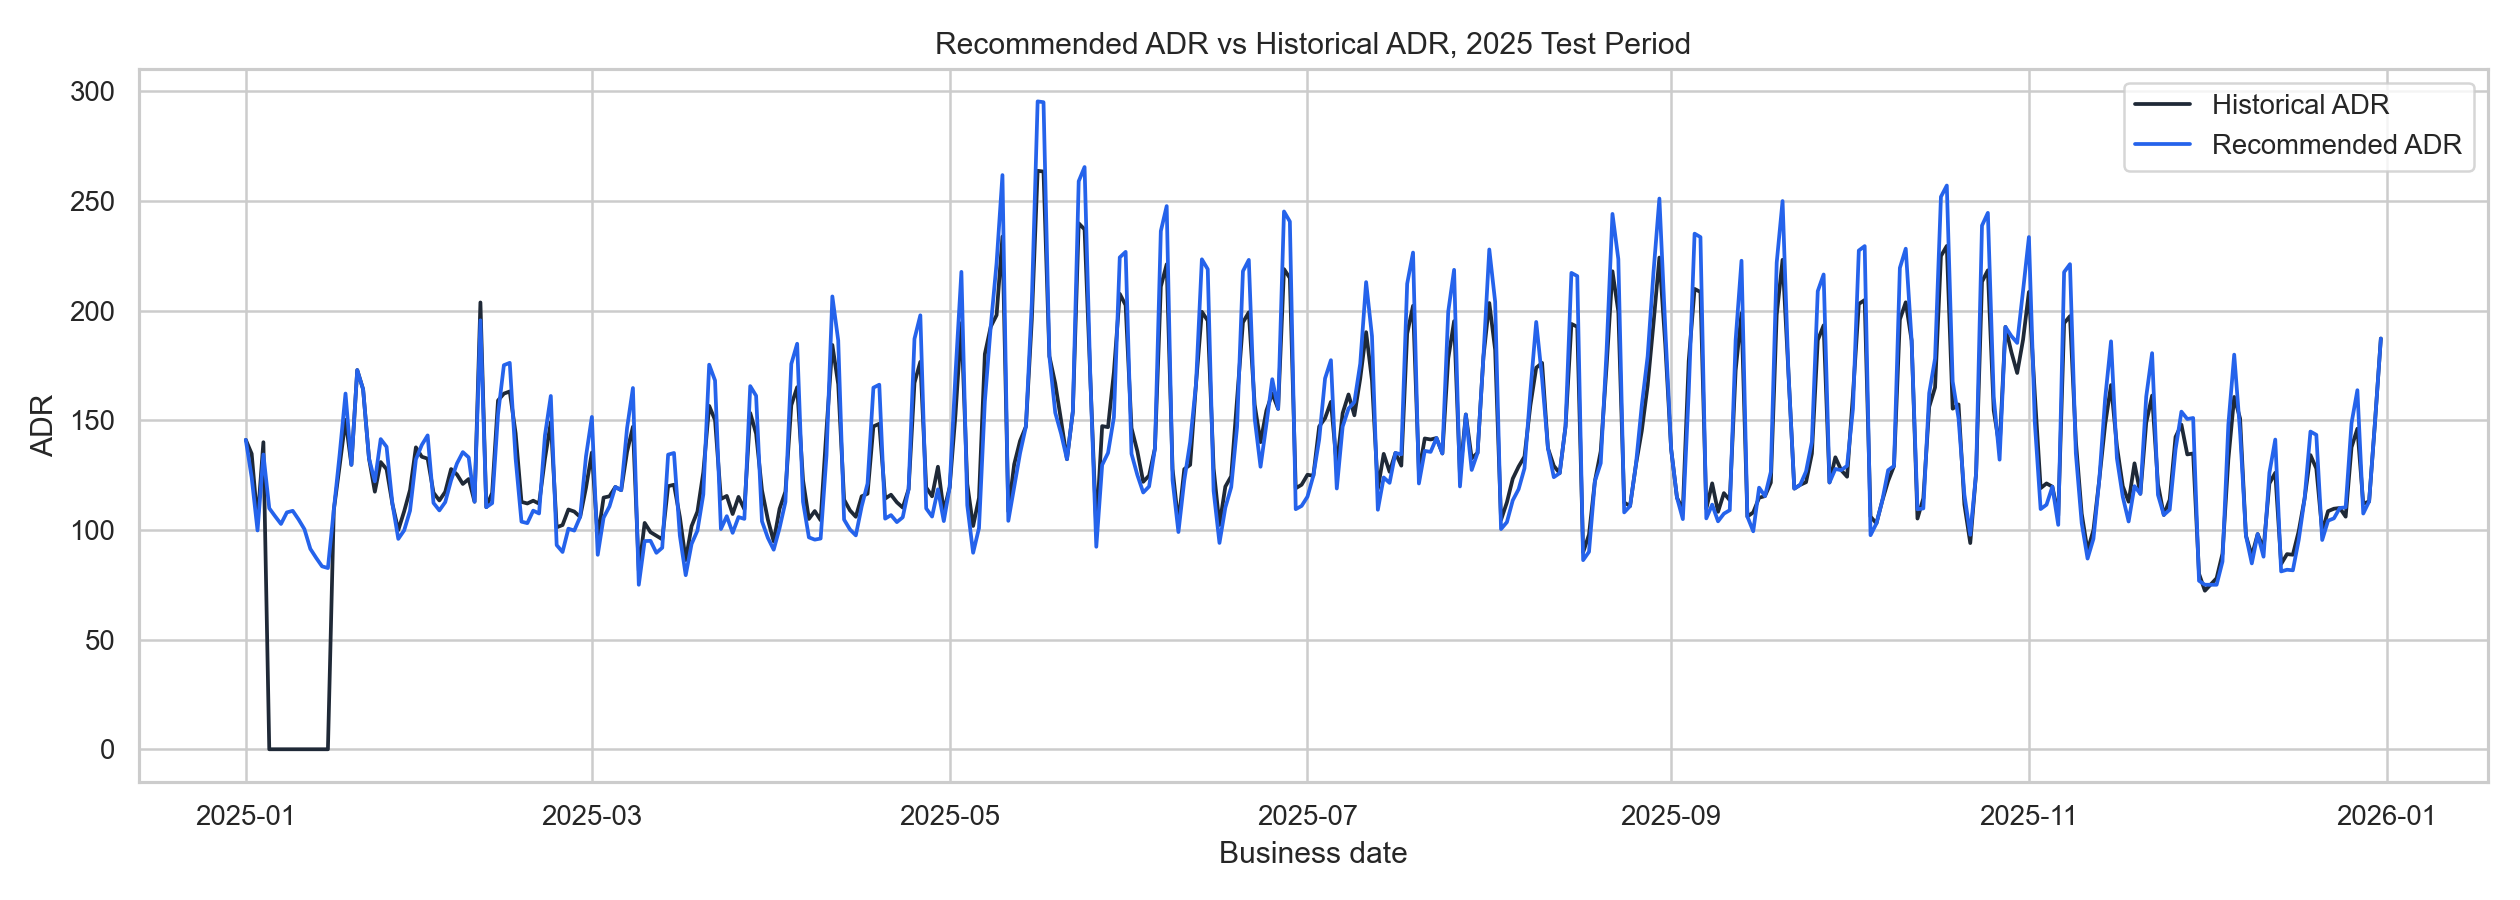
\includegraphics[width=\columnwidth]{pricing_recommended_vs_historical_adr.png}
    \caption{Recommended ADR versus historical ADR during the 2025 test period.}
    \label{fig:adr}
\end{figure}

\begin{figure}[t]
    \centering
    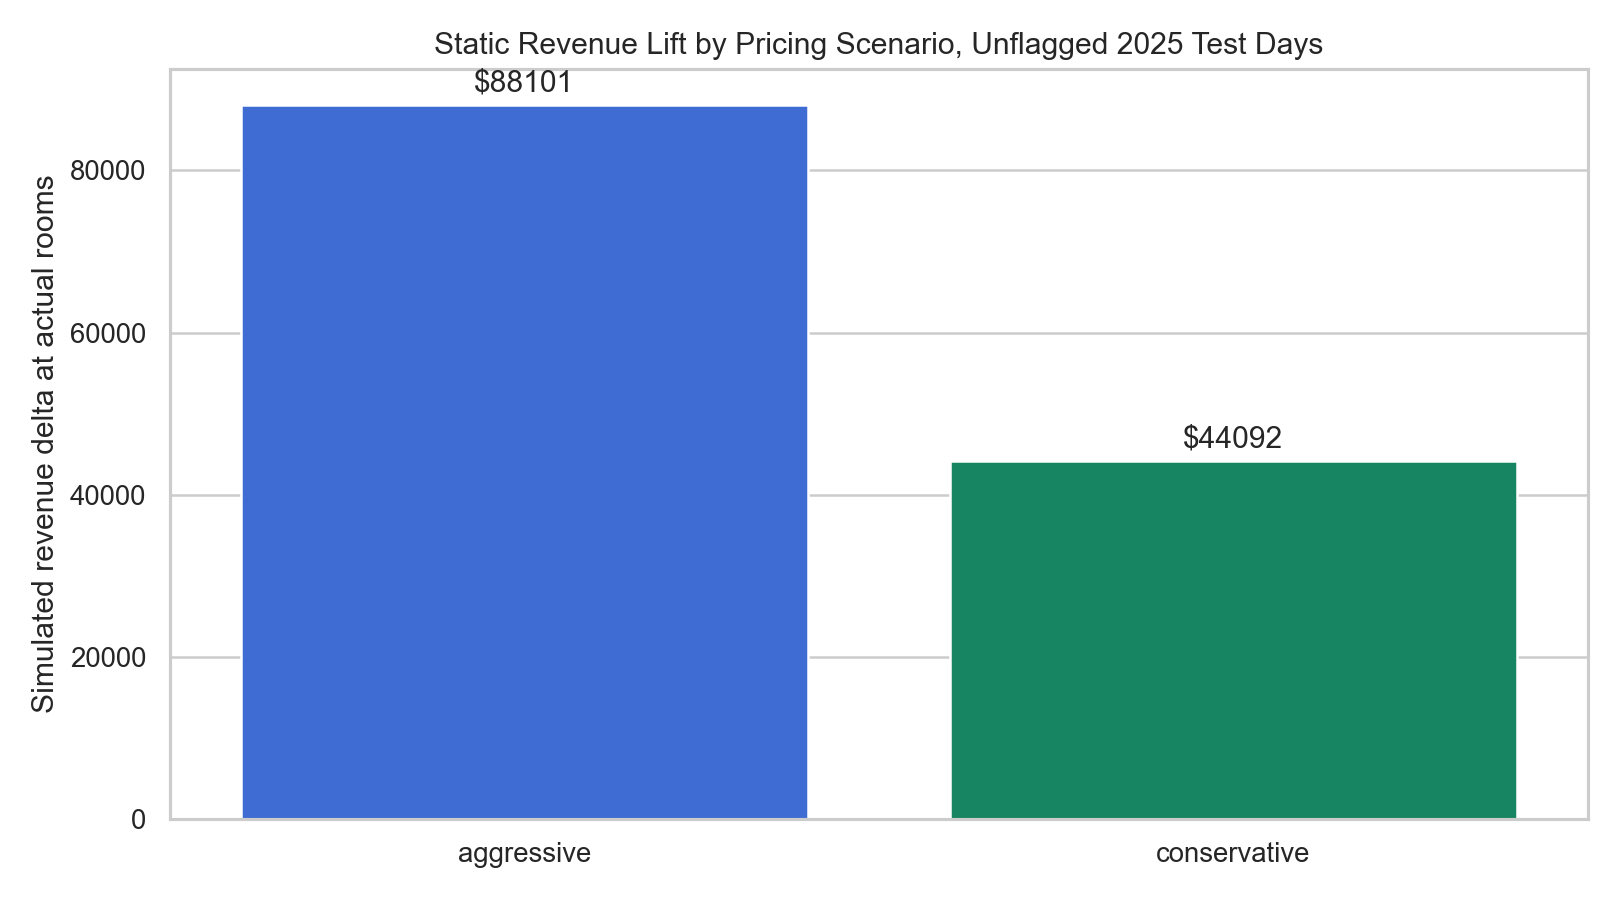
\includegraphics[width=\columnwidth]{pricing_scenario_comparison.png}
    \caption{Static simulated revenue lift by pricing scenario.}
    \label{fig:scenario}
\end{figure}

\section{High-Demand Scenario Examples}
To make the pricing recommendations concrete, Table~\ref{tab:examples} shows high-demand weekend dates from the unflagged 2025 test period. These dates have forecast occupancy near sellout levels and therefore receive upward ADR recommendations. For example, October 25, 2025 had 59 actual rooms sold and a forecast of 60.0 rooms; the aggressive rule recommends increasing ADR from \$218.36 to \$244.56, which yields a static simulated revenue delta of \$1,545.61.

\begin{table*}[t]
\centering
\caption{High-Demand Weekend Pricing Examples}
\label{tab:examples}
\begin{tabular}{llrrrrrr}
\toprule
Date & Day & Actual & Forecast & Hist. ADR & Agg. ADR & Cons. ADR & Agg. Delta\\
\midrule
2025-10-25 & Saturday & 59 & 60.0 & \$218.36 & \$244.56 & \$231.46 & \$1,545.61\\
2025-08-09 & Saturday & 57 & 60.0 & \$173.94 & \$194.81 & \$184.38 & \$1,189.38\\
2025-11-15 & Saturday & 59 & 60.0 & \$166.05 & \$185.98 & \$176.01 & \$1,176.15\\
2025-12-06 & Saturday & 60 & 60.0 & \$160.63 & \$179.91 & \$170.27 & \$1,156.63\\
2025-11-22 & Saturday & 58 & 60.0 & \$161.24 & \$180.59 & \$170.91 & \$1,122.11\\
2025-05-24 & Saturday & 57 & 59.9 & \$237.02 & \$265.46 & \$251.24 & \$1,621.31\\
\bottomrule
\end{tabular}
\end{table*}

\section{Limitations}
There are several limitations. First, the pricing simulation does not model demand response to price changes. A real revenue management system would need elasticity estimates, competitor pricing, channel mix, and customer response modeling. Second, some proposal features such as competitor prices and event indicators were only included if available; the final dataset did not contain a reliable external competitor or event feed. Third, booking lead time and booking pace were proposed as candidate features but are not engineered in the final model, because the only multi-record reservation source covers 2025 only and using it as training history would overlap with the held-out test period. Fourth, the proposal allowed either date-grain or date-room-type-grain modeling; the final implementation uses date-grain only because the available daily sample size already limits deep learning generalization, and a per-room-type breakdown would further fragment the signal. Fifth, January 2025 zero-room-sold dates were flagged as likely operational anomalies and should not be used as primary business evidence without verification. Finally, the dataset is small for deep learning: the best GRU and Transformer models get close, but the tabular tree models remain better suited to the available sample size.

\section{Conclusion}
This project implements the proposed hotel demand forecasting and pricing-support MVP end to end. The final system cleans operational reports, builds a daily modeling table, audits data quality, compares classical baselines against deep learning models, selects a primary demand model, and converts forecasts into bounded pricing recommendations.

The strongest forecasting result is XGBoost under the anomaly-excluded convention, with test MAE 7.443, RMSE 9.927, and $R^2$ 0.585. Deep learning models provide a meaningful comparison: the best GRU reaches MAE 7.813 and the best Transformer reaches MAE 7.835. Under a paired date-level bootstrap on the 354-row test set, the XGBoost advantage over Random Forest, the best GRU, and the best Transformer is not statistically significant at 95\% confidence, while the advantage over the best LSTM and best MLP is. The honest summary is therefore that the strongest tabular and sequence models tested form a statistical tie on this dataset, with LSTM and MLP variants trailing significantly. The pricing layer shows practical business potential under static assumptions, with simulated unflagged 2025 revenue lifts of 4.37\% for the aggressive scenario and 2.18\% for the conservative scenario.

Overall, the final recommendation is to use XGBoost as the MVP forecasting model. The justification is no longer purely accuracy-based: among the strongest models, accuracy ties at 95\% confidence under this paired date-level bootstrap, and XGBoost is selected because it is the most interpretable of the tied models and therefore the easiest for a revenue manager to audit and approve. GRU and Transformer results are presented as strong deep learning comparisons that match XGBoost's accuracy but require additional explanation tooling for operational use. The pricing layer is treated as a bounded decision-support tool rather than a complete commercial revenue management system.

\appendices

\section{Data Access and Property Notes}
\label{app:property}
The 60-room inventory figure is consistent across every operational reporting period in the dataset and is used directly as the property capacity throughout the modeling and pricing pipeline. The two over-capacity rows flagged in the data-quality audit correspond to dates where the source report shows rooms sold above 60, which is mechanically impossible given the inventory and is therefore treated as an operational reporting anomaly rather than real demand.

My family connection to a partner at the property made it possible to use this particular dataset for an academic project. The raw operational workbooks and the cleaned and processed CSVs derived from them are \textbf{not publicly available}, because they contain commercially sensitive single-property revenue history (rooms sold, ADR, RevPAR, net room revenue) as well as guest personally identifiable information (names, emails, comments, confirmation and folio numbers) drawn from the property's reservation system. For these reasons \texttt{Data/}, \texttt{cleaned\_data/}, and \texttt{processed\_data/} are excluded from the public repository via \texttt{.gitignore} and are not redistributed. The modeling code, evaluation harness, pricing layer, and report-generation pipeline are fully open at the repository linked in Appendix~\ref{app:repo}, and PII is excluded from all modeling artifacts. To make the data shape inspectable without releasing the underlying data, sanitized synthetic example CSVs that share only the column schema of the cleaned and processed files are provided in the public \texttt{data\_examples/} folder; these are referenced in Appendix~\ref{app:examples}.

\section{Repository, Reproduction, and Artifacts}
\label{app:repo}
The full source code, cleaning scripts, modeling pipeline, pricing layer, and report artifacts are publicly available at \url{https://github.com/jackdemarinis/CSC_561_Final_Project}. The data directories \texttt{Data/} (raw operational workbooks), \texttt{cleaned\_data/} (cleaned outputs), and \texttt{processed\_data/} (derived modeling features) are present locally but are excluded from the public repository via \texttt{.gitignore} for the privacy reasons described in Appendix~\ref{app:property}. Sanitized schema-only example CSVs for these folders ship in \texttt{data\_examples/} (see Appendix~\ref{app:examples}). Metrics, figures, and the IEEE report live under \texttt{reports/}. Source code is split under \texttt{src/} into feature construction, model training, evaluation, and pricing. Tables and figures in the paper are generated from the same CSV and JSON artifacts produced by the scripts when the pipeline is rerun against private hotel exports of the same shape.

The reproduction order is: clean operational exports (\texttt{scripts/clean\_new\_operational\_reports.py}); build guest daily enrichment and the date-grain modeling table (\texttt{src/features/}); audit data quality (\texttt{src/evaluation/audit\_modeling\_data\_quality.py}); train baselines, run sensitivity, and train deep learning models (\texttt{src/models/}, \texttt{src/evaluation/run\_baseline\_sensitivity.py}); build pricing recommendations (\texttt{src/pricing/}); and compile \texttt{reports/final/final\_report\_ieee.tex}. The central artifact is \texttt{processed\_data/modeling\_daily.csv}: 1,096 daily rows from 2023-01-01 through 2025-12-31, with no missing or duplicate business dates. Train ends 2024-06-30; validation runs through 2024-12-31; test is calendar year 2025.

Result tables and figures map directly to subfolders: \texttt{reports/audit/} for data-quality flags, \texttt{reports/baselines/} and \texttt{reports/deep\_learning/} for model metrics, \texttt{reports/pricing/} for ADR recommendations and business metrics, and \texttt{reports/figures/} for PNG figures. Inspecting those CSV/JSON files is the quickest way to check whether the PDF has drifted from current code output.

\section{Data Sources and Modeling Policy}
\subsection{Data Sources}
Three operational families feed the modeling table. Block RoomSales (2023--2025) provides daily property-level rooms sold, revenue, ADR, RevPAR, and inventory; reconciliation checks confirm room-type rows plus deduplicated adjustment rows tie to property daily totals, and inferred hotel inventory is 60 rooms throughout. ReservationForecast files (2023--2024) overlap exactly with Block on rooms sold, out-of-order rooms, and net room revenue, but use a different occupancy denominator (sellable rooms vs.\ total inventory); both definitions are kept as explicit columns rather than collapsed. GuestNameList exports are 2025-only reservation reports parsed into 10,579 deduplicated stay-like records. Guest PII (names, emails, confirmation/folio numbers) is used only for cleaning and deduplication and is excluded from modeling features; the daily enrichment aggregates to non-identifying counts, shares, and rates.

\subsection{Feature Policy and Leakage Control}
The forecasting task uses calendar features (date fields, cyclical day-of-week, month, and day-of-year encodings), lag features at 1, 7, 14, 28, and 365 days, and rolling windows over 7, 14, 28, and 56 days, all over rooms sold, net ADR, net room revenue, and reported occupancy. Same-day Block fields, raw ReservationForecast fields, same-day guest enrichment, and source lineage columns are blocked from learned model inputs unless they appear only as lagged or rolling historical versions. Guest-derived features are also treated cautiously because the guest-list source mainly covers 2025 and is not a complete multi-year historical signal. This leakage policy is the most important experimental safeguard in the repository.

\subsection{Data-Quality Sensitivity}
Fourteen anomaly rows are flagged in the modeling table: twelve zero-room-sold dates and two rows where rooms sold exceed the 60-room inventory. The primary \texttt{exclude\_all\_flagged} convention drops all fourteen, leaving 354 test rows in 2025. The decision-level sensitivity is stable: XGBoost is best by MAE under both the exclude-all-flagged and full-data conventions, and Random Forest is best under the over-capacity-only convention. Random Forest is sometimes stronger by RMSE or $R^2$, which is why both tree models remain visible in the main comparison.

\section{Pricing Layer Notes}
The pricing layer is a bounded decision-support rule, not a revenue management optimizer. It starts from the selected XGBoost forecast, converts forecast rooms sold into forecast occupancy against the 60-room inventory, assigns a demand band, and adjusts a reference ADR drawn from historical same-day net ADR with rolling, lagged, and median fallbacks. Recommendations are bounded by minimum ADR, maximum ADR, and a 20\% daily move cap from the reference. Two scenarios (aggressive and conservative) are reported because a single pricing curve would imply false precision; both are static counterfactuals applied to actual realized rooms sold and do not model price elasticity, competitor reaction, or channel mix.

A production version would need at least four extensions: (i) elasticity estimates or controlled experiments so ADR changes affect expected rooms sold rather than being applied to fixed history; (ii) competitor-rate, local-event, and holiday-demand feeds; (iii) error monitoring by day of week, occupancy band, month, and high-demand period; and (iv) human approval for flagged dates, unusually large ADR moves, and near-sellout dates. The current system can identify days when historical signals suggest higher or lower occupancy pressure and translate that into bounded ADR advice; it cannot yet answer whether a specific ADR change maximizes profit after customer response, cancellations, competitor movement, and distribution costs.

\section{Sanitized Data Schema Examples}
\label{app:examples}
Because the raw, cleaned, and processed data files are not publicly available (Appendix~\ref{app:property}), the public repository ships a \texttt{data\_examples/} folder containing synthetic, sanitized CSVs that reproduce the column schema of each pipeline output. Every value in these example files is fabricated; no real business date, real rooms sold, real ADR, real revenue, or real guest record appears in any of them. They are intended only as a reference so that a reader can see the column names, column ordering, and column dtypes that the open-source pipeline expects and produces.

\begin{table}[h]
\centering
\caption{Public Schema Examples in \texttt{data\_examples/}}
\label{tab:examples_files}
\resizebox{\columnwidth}{!}{%
\begin{tabular}{ll}
\toprule
Example file (synthetic) & Mirrors private file\\
\midrule
\texttt{block\_roomsales\_daily\_totals\_example.csv} & \texttt{cleaned\_data/block\_roomsales\_daily\_totals\_cleaned.csv}\\
\texttt{block\_roomsales\_room\_type\_daily\_example.csv} & \texttt{cleaned\_data/block\_roomsales\_room\_type\_daily\_cleaned.csv}\\
\texttt{block\_roomsales\_room\_class\_daily\_example.csv} & \texttt{cleaned\_data/block\_roomsales\_room\_class\_daily\_cleaned.csv}\\
\texttt{block\_roomsales\_adjustments\_example.csv} & \texttt{cleaned\_data/block\_roomsales\_adjustments\_cleaned.csv}\\
\texttt{reservation\_forecast\_daily\_example.csv} & \texttt{cleaned\_data/reservation\_forecast\_daily\_cleaned.csv}\\
\texttt{guest\_stays\_example.csv} & \texttt{cleaned\_data/guest\_stays\_cleaned.csv} (PII redacted)\\
\texttt{guest\_daily\_enrichment\_example.csv} & \texttt{processed\_data/guest\_daily\_enrichment.csv}\\
\texttt{modeling\_daily\_example.csv} & \texttt{processed\_data/modeling\_daily.csv}\\
\bottomrule
\end{tabular}}
\end{table}

The example files contain the full column header of each cleaned or processed dataset together with one to three synthetic data rows demonstrating the expected value types (dates, integer counts, float rates, share fractions in $[0,1]$, and categorical strings). The PII columns of the guest-stays schema (\texttt{guest\_name}, \texttt{email}, \texttt{comments}, \texttt{confirmation\_number}, \texttt{folio\_number}, \texttt{room\_number}) are present in the example header for completeness but are populated only with placeholder tokens such as \texttt{REDACTED\_NAME} and \texttt{redacted@example.invalid}. These columns never enter the modeling features (Appendix~\ref{app:property}); the modeling table consumes only the daily aggregates produced by \texttt{src/features/build\_guest\_daily\_enrichment.py}, whose schema is shown in \texttt{guest\_daily\_enrichment\_example.csv}. A reader with access to comparable hotel operational exports can run the open-source pipeline unchanged against their own data and reproduce files matching these schemas.

\bibliographystyle{IEEEtran}
\bibliography{references}

\end{document}
